\section{Introduction}
Vessel diseases are among the most common causes of death according to the WHO. Calcifications and soft plaque are occurring and hinder the blood flow through affected areas. \cite{WHO2017} Though, the proper analysis of vessels within the human body is a rather time consuming task, since the images created need to be analyzed from multiple angles. Curvicircular Feature Aggregation (CFA), makes this quicker and more error resistant by removing the need of analyzing a vessel from all sides.

\section{Algorithm}
The algorithm needs three dimensional image data from the vessels to be analyzed. Additionally contrast agent should be applied so that the vessel are brighter then the normal tissue but less intense then bones and calcifications. The algorithm is concluded from \cite{Mistelbauer2013}.

Figure 1 shows the steps made to process the data and create a CFA image.

\begin{figure} \label{img_workflow}
	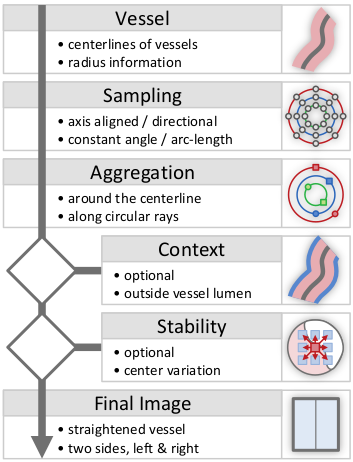
\includegraphics[width=\columnwidth]{img/cfaworkflow}
	\caption{The steps of the algorithm in order \cite{Mistelbauer2013}.}
\end{figure}

\subsection{Vessel data}
The algorithms needs centerlines of the vessels and radii provided to function. If the radii are not given it is possible to either estimate them or ignore the contextual imaging.

\subsection{Sampling}
Circular concentric rays are cast around the centerpoints of each slice. On every ray multiple samples are taken from the image data. The amount of samples can be defined by either a \textbf{fixed angle} or \textbf{fixed arc length}. Note that with fixed arc length the amount of samples for bigger circles increases which results in a higher amount of computational power needed. The set of sample points may be defined as:

\begin{equation}
S_{n,X,r,s} = \{X + R \cdot (cos(i \cdot \frac{2\pi}{n})\cdot r + sin(i \cdot \frac{2\pi}{n}) \cdot s)\}
\end{equation}

With $n$ being the amount of samples taken, $X$ as the observed center point and $R$ the radius of the analyzed circular ray. $r$ and $s$ are the plane projecting vectors and therefore orthogonal on each other and the vessel.
\begin{figure*}
	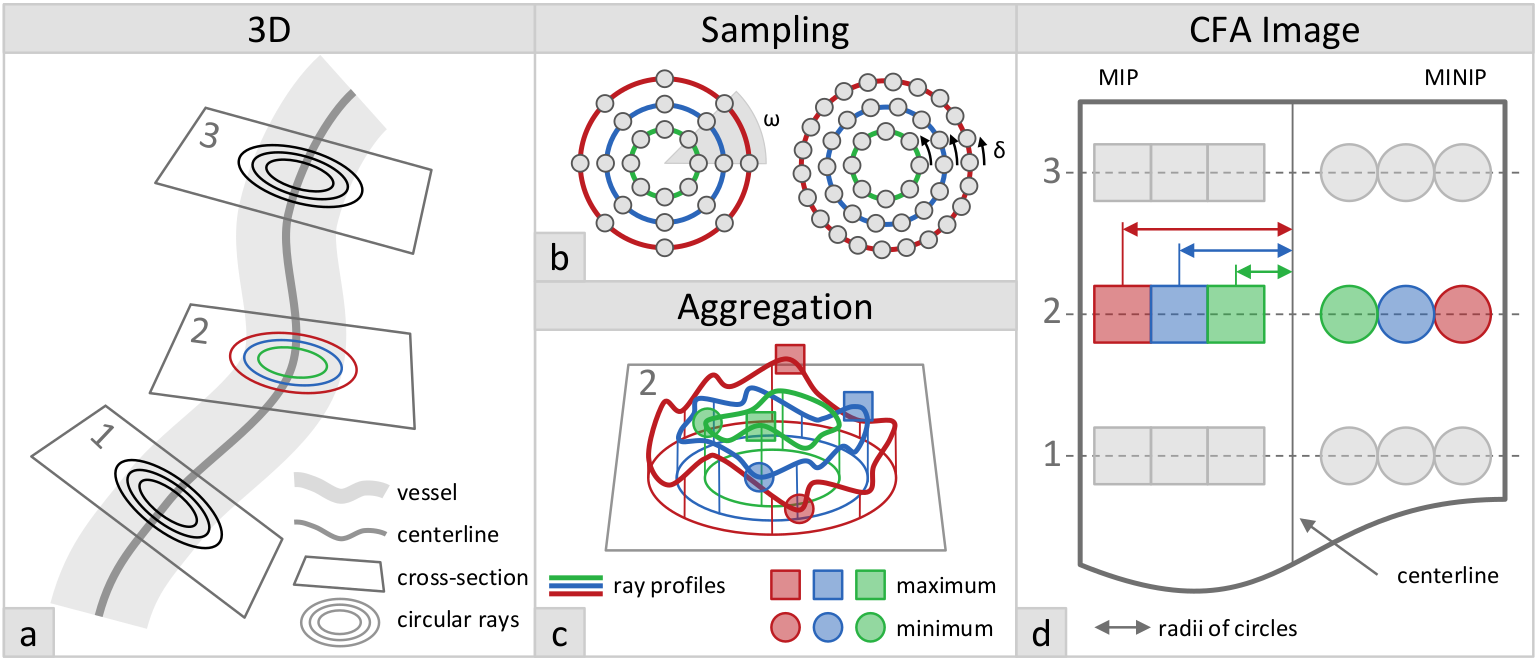
\includegraphics[width=2\columnwidth]{img/cfasampling}
	\caption{The generation of the CFA images visualized. \textbf{a} describes how the data is structured with the centerline and the concentric samples. \textbf{b} compares constant-angle and constant-arc-length sampling. \textbf{c} visualizes the search for minima and maxima. \textbf{d} show how the image is finally constructed with the data from \textbf{c} \cite{Mistelbauer2013}.}
\end{figure*}

\subsection{Aggregation}
Every aggregation function which does not take the order of the samples in account can be used to evaluate the data. \textbf{Average} or \textbf{Median} calculations are possible, but are not really medically relevant. Instead \textbf{Maximum} and \textbf{Minimum} intensity projections (abbreviated MIP and MINIP respectively) are made. This means, that for each circular ray the minimum and maximum of the samples are determined and visualized. The proposed method is to have the center point in the middle of the image, the maximum to the left and the  minimum to the right.

\subsection{Context}
Since the CFA does not give relevant information outside of the vessel, the image beyond this area can be visualized differently. This view may be either rotated or just be a fixed frontal view of the data. This means casting linear rays through the body and creating an equivalent MIP or MINIP. This results in our final image to be calculated as:

\begin{equation}
I_F(x,y)= 
\begin{cases}
I_{CFA},& \text{if } |x_{cl} - x | \le R_{max} \cdot f \\
I_{CTX},& \text{if } |x_{cl} - x | > R_{max} \cdot f
\end{cases}
\end{equation}

Where $f$ is a constant value greater one to make sure the contextual data is only used outside the vessel if the radius information is not precise.

\subsection{Stability}

The stability of the centerline which can be seen as the centeredness. This factor is really important since, minor errors can result in false analysis of the CFA images. For every point $C$ the neighborhood with \textit{"range"} $w$ is defined as:

\begin{equation}
N_{C,w} = \{C + i \cdot r\} \times \{C + j \cdot s\}
\end{equation}

$w$ is user-specified, note that the algorithm is in $O(w^2)$ and therefore larger values of $w$ will result in longer runtime. $r$ and $s$ are again the plane projecting vectors of the orthogonal plane of the vessel. The variance of the neighborhood is then mapped to a red color if high. A high variance near to the center line is equivalent to a low stability and vice versa.

\subsection{Result}
A result image can look like Figure 3. 
\begin{figure}
	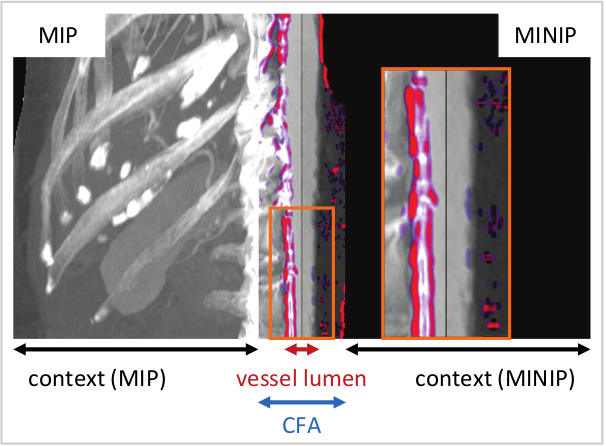
\includegraphics[width=\columnwidth]{img/cfaresult}
	\caption{Visualization of a vessel using CFA, context information and stability calculation in the human body \cite{Mistelbauer2013}.}
\end{figure}
Contrast agent is applied, therefore the vessel is gray colored. The bones in the context information and the calcifications are white visualized on the MIP side (left). Soft plaque and stenosis is seen in the MINIP projection (right).

\section{Conclusion}
The algorithm reduced the needed interaction when analyzing vessel image data. The original authors asked nine radiologists to give them their opinion about the information and the visualization of CFA. Their opinions are shown in Figure 4.
\begin{figure}
	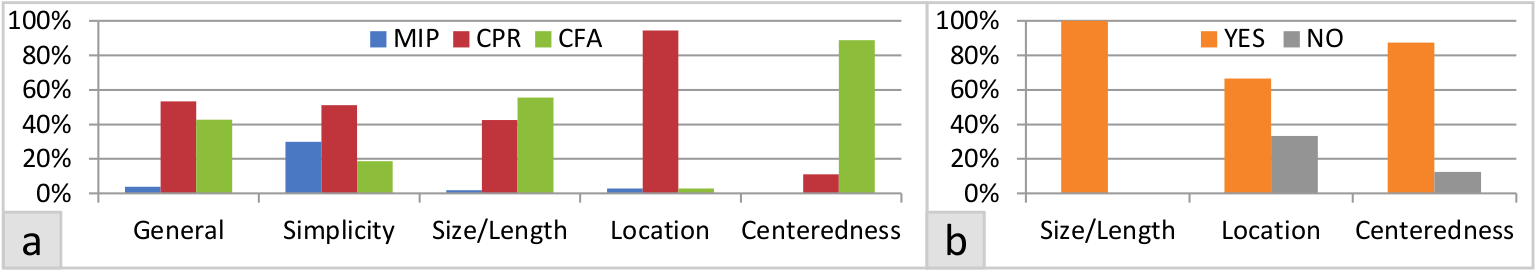
\includegraphics[width=\columnwidth]{img/cfaeval}
	\caption{Evaluation of 9 radiologists. \textbf{a} describes their evaluation on how good an algorithm is for a given type of information. \textbf{b} visualizes whether a type of information is important for them \cite{Mistelbauer2013}.}
\end{figure}

